\part[author={\protect\insertauthor}]{Lexical Analysis}
\label{chap:lexical_analysis}

\begin{graphicspathcontext}{{./chapters/chapter2/imgs/auto/}}
\begin{bibunit}[apalike]
	
\tableofcontentslide

\section{Introduction}

\tableofcontentslide[sections={1-5},sectionstyle={show/shaded},subsectionstyle={show/show/hide},subsubsectionstyle={hide/hide/hide/hide}]

\subsection{General principles}
\begin{frame}{Lexical Analyzer}
	\alertbox{The lexical analyzer reads the stream of characters making up the source program.}
	\begin{itemize}
	\item It groups the characters into meaningful sequences called \emph{lexemes}.
	\item For each lexeme, the lexical analyzer produces as output a \emph{token} of the following form; and passes it to the syntactic analyzer.
		\begin{center}
			\code{{\textless}token-name, attribute-value{\textgreater}}
		\end{center}
	\item The \code{token-name} is the identifier of the token.
	\item The \code{attribute-value} points to an entry in the symbol table for this token.
	\end{itemize}
\end{frame}

\begin{frame}{Lexical Analyzer}
	\begin{itemize}
	\item The tasks of the lexical analyzer of a compiler are: \begin{enumerate}
		\item discovering the tokens,
		\item stripping the blanks and the comments,
		\item correlating the error messages with the source program (line number tracking\dots)
		\end{enumerate}
	\vspace{1em}
	\item Sometimes, lexical analyzers are divided into a cascade of two processes: \begin{description}
		\item[Scanning] consists of the simple processes that do not require tokenization of the input: deletion of comments and compaction of consecutive white spaces.
		\item[Lexical analysis] is the more complex portion, which produces tokens from the output of the scanner.
		\end{description}
	\end{itemize}
\end{frame}

\subsection{Definitions}
\begin{frame}{Lexeme}
	\begin{itemize}
	\item A \emph{lexeme} is a sequence of characters in the source program that is identified by the lexical analyzer as a lexical unit (element of the language).
	\end{itemize}
	\vfill
	\begin{example}
		\begin{itemize}
		\item Let the statement: \code{\id{printf}(\str{"Total = \%d{\textbackslash}n"}, \id{score});}
		\item Both \id{printf} and \id{score} are lexemes.
		\item The string of characters is a lexeme.
		\item The parenthesis, coma and semicolumn characters are also lexemes.
		\end{itemize}
	\end{example}
\end{frame}

\begin{frame}{Token}
	\begin{itemize}
	\item A \emph{token} is a pair consisting of a token name and an optional attribute value.
	\item The token name is an abstract symbol representing a kind of lexical unit.
	\item The token names are the input symbols that the parser processes.
	\item Generally the tokens are written in \tok{boldface}.
	\end{itemize}
	\vfill
	\begin{example}
		\begin{itemize}
		\item Let the statement: \code{\id{printf}(\str{"Total = \%d{\textbackslash}n"}, \id{score});}
		\item both \id{printf} and \id{score} are lexemes matching the pattern for token \tok{id}.
		\end{itemize}
	\end{example}
\end{frame}

\begin{frame}{Pattern}
	\begin{itemize}
	\item A \emph{pattern} is a description of the form that the lexemes of a token may take.
	\item In the case of a keyword as a token, the pattern is just the sequence of characters that form the keyword.
	\item For identifiers and some other tokens, the pattern is a more complex structure that is \emph{matched} by many strings.
	\end{itemize}
	\vfill
	\begin{example}
		\begin{itemize}
		\item Let the statement: \code{\id{printf}(\str{"Total = \%d{\textbackslash}n"}, \id{score});}
		\item both \id{printf} and \id{score} are described by the pattern \code{[\_a-zA-Z][\_a-zA-Z]*}
		\end{itemize}
	\end{example}
\end{frame}

\begin{frame}{Classes of Tokens}
	In many programming languages, the following classes cover most or all of the tokens:
	\begin{enumerate}
	\item One token for each keyword. The pattern is the name of the token itself;
	\item Tokens for the operators, either individually or in classes such as the token \tok{comparison};
	\item One token representing all identifiers;
	\item One or more tokens representing constants, such as numbers and literal strings;
	\item Tokens for each punctuation symbol, such as left and right parentheses, comma, and semicolon.
	\end{enumerate}
\end{frame}

\begin{frame}{Attributes of Tokens}
	\begin{itemize}
	\item When more than one lexeme can match a pattern, the lexical analyzer must provide to the subsequent compiler phases additional information about the particular lexeme that matched.
For example: the token \tok{number} matches 0 and 1234.
	\item The lexical analyzer returns to the parser the token name and an attribute value that describes the lexeme represented by the token.
	\item We shall assume that tokens have at most one associated attribute. But it could be a data structure.
		\begin{example}
		The attribute value for the token \tok{id} is an entry in the symbol table.
		\end{example}
	\end{itemize}
\end{frame}

\subsection{Separating the lexical analyzer and the parser}
\begin{frame}{Lexical Analyzer and Parser}
	\begin{itemize}
	\item The lexical analyzer generally does not control the execution flow of the compiler.
	\vfill
		\begin{center}
			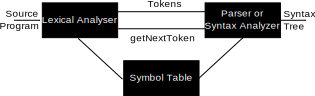
\includegraphics[width=.9\linewidth]{lexical_parser_relation}
		\end{center}
	\vfill
	\item The lexical analyzer is invoked by the parser through a call to \code{getNextToken}.
	\item Then the lexical analyzer tries to discover and to reply a token.
	\end{itemize}
\end{frame}

\begin{frame}{Why Separating Lexical Analyzer and Parser?}
	There are number of reasons why the lexical analysis and the parsing are separated:
	\begin{description}
	\item[Simplicity of design] The separation of lexical and syntactic analysis often allows us to simplify at least one of these tasks.
	\vfill
	\item[Compiler efficiency] A separate lexical analyzer allows us to apply specialized techniques.
	\vfill
	\item[Compiler portability] Input-device-specific peculiarities can be restricted to the lexical analyzer.
	\end{description}
\end{frame}

\subsection{Lexical errors}
\begin{frame}{Lexical Errors}
	\begin{itemize}
	\item It is hard for a lexical analyzer to tell that there is a source-code error.
	\vfill
	\item Let: \code{fi ( a == f(x)) \dots}
	\vfill
	\item The lexical analyzer cannot tell whether \code{fi} is a misspelling of the keyword \kw{if} or an undeclared function identifier.
	\vfill
	\item The lexical analyzer fails when none of the patterns for tokens matches any prefix of the remaining input.
	\vfill
	\item If such an error is detected, the lexical analyzer must output an error message, and try to recover a stable state.
	\end{itemize}
\end{frame}

\begin{frame}{Recovery Strategies}
	\begin{itemize}
	\item The simplest recovery strategy is the ``\emph{panic mode}.''
		\begin{itemize}
		\item We delete successive characters from the remaining input, until the lexical analyzer can find a well-formed token at the beginning of what input is left.
		\end{itemize}
	\vfill
	\item Other possible error-recovery actions are:
		\begin{itemize}
		\item Delete one character from the remaining input.
		\item Insert a missing character into the remaining input.
		\item Replace a character by another character.
		\item Transpose two adjacent characters.
		\end{itemize}
	\end{itemize}
\end{frame}

\section{Input buffering}

\tableofcontentslide[sectionstyle={show/shaded},subsectionstyle={show/show/hide},subsubsectionstyle={hide/hide/hide/hide}]

\begin{frame}{Reading the Source Program}
	\begin{itemize}
	\item The task of reading the source program is important and may be time consuming. It must be accelerated.
	\vfill
	\item This task is made difficult by the fact that we often have to look one or more characters beyond the next lexeme before we can be sure we have the right lexeme.
	\vfill
	\item For instance, we cannot be sure we have seen the end of an identifier until we see a character that is not a letter or a digit, and therefore is not part of the lexeme for \tok{id}.
	\vfill
	\item \emph{We shall introduce a two-buffer scheme that handles large lookaheads safely.}
	\end{itemize}
\end{frame}

\pgfdeclareimage[width=.7\paperwidth]{buffer_pair_example}{./chapters/chapter2/imgs/auto/buffer_pair_example}

\begin{frame}[t]{Using a Pair of Buffers}
	\begin{itemize}
	\item Specialized buffering techniques have been developed to reduce the amount of overhead required to process a single input character.
	\vfill
	\item An important scheme involves two buffers that are alternatively reloaded:
		\begin{center}
		{\pgfuseimage{buffer_pair_example}}
		\end{center}
	\vfill
	\item Each buffer is of the same size $N$ (usually the size of the disk block).
	\vfill
	\item Using one \emph{system read command}, we can read $N$ characters into a buffer, rather than a call per character.
	\end{itemize}
\end{frame}

\begin{frame}[t]{Using a Pair of Buffers}
	\begin{itemize}
	\item A special character (\tok{eof}) is put in the buffer when there is not enough characters in the input.
	\vfill
	\item Two pointers to the input are maintained: \begin{itemize}
		\item Pointer \id{lexemeBegin}, marks the beginning of the current lexeme, whose extent we are attempting to determine.
		\item Pointer \id{forward} scans ahead until a pattern match is found.
		\end{itemize}
	\end{itemize}
	\vfill
	\begin{center}
	{\pgfuseimage{buffer_pair_example}}
	\end{center}
\end{frame}

\begin{frame}[t]{Using a Pair of Buffers}
	\begin{description}
	\item Once the next lexeme is determined, \id{forward} is set to the character at its right.
	\item When the lexeme is recorded as an attribute value of a token, the \id{lexemeBegin} is set to the character immediately after the lexeme just found.
	\item When \id{forward} is outside a buffer, the other buffer is reloaded from the input, and move \id{forward} to the beginning of the newly loaded buffer.
	\item[Assumption] the larger lexeme has a size lower or equals to $N$.
	\end{description}
	\vfill
	\begin{center}
	{\pgfuseimage{buffer_pair_example}}
	\end{center}
\end{frame}

\begin{frame}{Can We Run Out Of Buffer Space?}
	\begin{itemize}
	\item In most modern languages, lexemes are short. Thus a buffer size $N$ in the thousands is ample, and the double-buffer scheme works without problem.
	\vfill
	\item But some problems may occurs: character strings can be very long, extending over many lines, then we could face the possibility that a buffer overflow occurs.
	\vfill
	\item To avoid problems with long character strings, we can: \begin{description}
		\item add a dynamic buffer scheme for large lexeme; or
		\item reply to the parser a sequence of \tok{str} tokens, one for each of the shorter strings.
		\begin{example}
			compile-time string concatenation in C: \code{\str{"ABC"} \str{"DEF"}}
		\end{example}
		\end{description}
	\end{itemize}
\end{frame}

\begin{frame}{Sentinels}
	\begin{itemize}
	\item According to the previously described double-buffer scheme, for each character read, we make two tests: \begin{description}
		\item one for the end of the buffer, and
		\item one to determine what character is read (usually a multiway branch).
		\end{description}
	\item To improve the speed of the treatment, we can combine the two tests by extending each buffer with a \emph{sentinel character} (usually \tok{eof}).
	\end{itemize}
	\vfill
	\begin{center}
		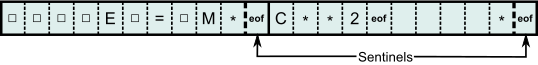
\includegraphics[width=\linewidth]{buffer_pair_sentinel_example}
	\end{center}
\end{frame}

\section[Token Recognition]{Specification and recognition of tokens}

\tableofcontentslide[sections={1-5},sectionstyle={show/shaded},subsectionstyle={show/show/hide},subsubsectionstyle={hide/hide/hide/hide}]

\subsection{Strings and operations on languages}
\begin{frame}{Strings and Languages}
	\begin{itemize}
	\item An \emph{alphabet} is any finite set of symbols. \\
		\inlineexample{$A = \left\{a,b,c,\delta\right\}$}
	\vfill
	\item A \emph{string} over an alphabet is a finite sequence of symbols drawn from that alphabet. \\
		\inlineexample{$s \in S=\permut(\powerset(A)) \setminus \{\emptyset\} = \left\{a,b,c,\delta,ab,ac,a\delta,\dots\right\}$}
	\item The length of a string $s$, usually written $|s|$, is the number of occurrences of symbols in $s$.
	\vfill
	\item A \emph{language} is any countable set of strings over some fixed alphabet. \\
		\inlineexample{$L \subseteq S = \left\{abc,\delta,b,bc\right\}$}
	\end{itemize}
\end{frame}

\sidecite{Kleene.1956}
\begin{frame}[c]{Operations on Languages}
	\begin{block}{Union of the languages $L$ and $M$}
		$L \cup M = \left\{s | s\in L \vee s \in M\right\}$
		\begin{tabularx}{\linewidth}{@{}lX@{}}
		\insertexamplelabel & Let $L = \left\{ a, b ,c \right\}$ and $M = \left\{ d, e \right\}$ \\
		& then $L \cup M = \left\{ a, b, c, d, e \right\}$
		\end{tabularx}
	\end{block}
	\begin{block}{Concatenation of the languages $L$ and $M$}
		$LM = \left\{st | s\in L, t \in M\right\}$
		\begin{tabularx}{\linewidth}{@{}lX@{}}
		\insertexamplelabel & Let $L = \left\{ a, b ,c \right\}$ and $M = \left\{ d, e \right\}$ \\
		& then $L \cup M = \left\{ ad, ae, bd, be, cd, ce \right\}$
		\end{tabularx}
	\end{block}
\end{frame}

\sidecite{Kleene.1956}
\begin{frame}[c]{Operations on Languages}
	\begin{block}{Self-concatenation of the language $L$}
		$L^i = \begin{cases}
			\{\epsilon\} & \text{if }i=0 \\
			L^{i-1}L & \text{if }i>0 \\
			\end{cases}$
		\begin{tabularx}{\linewidth}{@{}lX@{}}
		\insertexamplelabel & Let $M = \left\{ d, e \right\}$ \\
		& then $M^4 = \left\{ \begin{array}{l}
			\scriptstyle dddd, ddde, ddded, ddee, dedd, dede, \\
			\scriptstyle deded, deee, eddd, edde, edded, edee, \\
			\scriptstyle eedd, eede, eeded, eeee \end{array} \right\}$
		\end{tabularx}
	\end{block}
\end{frame}

\sidecite{Kleene.1956}
\begin{frame}[c]{Operations on Languages}
	\begin{block}{Kleene's Closure of the language $L$}
		$L^* = \bigcup^{\infty}_{i=0}L^i$
		\begin{tabularx}{\linewidth}{@{}lX@{}}
		\insertexamplelabel & Let $M = \left\{ d, e \right\}$ \\
		& then $M^* = \left\{ \begin{array}{l}
			\scriptstyle \epsilon, d, e, dd, de, ed, ee, ddd, dde, ded, dee, edd, ede, eed, \\
			\scriptstyle eee, dddd, ddde, dded, ddee, dedd, dede, deed, deee, \dots\end{array} \right\}$
		\end{tabularx}
	\end{block}
	\begin{block}{Positive Closure of the language $L$}
		$L^+ = \bigcup^{\infty}_{i=1}L^i$
		\begin{tabularx}{\linewidth}{@{}lX@{}}
		\insertexamplelabel & Let $M = \left\{ d, e \right\}$ \\
		& then $M^+ = \left\{ \begin{array}{l}
			\scriptstyle d, e, dd, de, ed, ee, ddd, dde, ded, dee, edd, ede, eed, \\
			\scriptstyle eee, dddd, ddde, dded, ddee, dedd, dede, deed, \dots\end{array} \right\}$
		\end{tabularx}
	\end{block}
\end{frame}

\subsection{Regular expressions}

\tableofcontentslide[sections={1-5},sectionstyle={show/shaded},subsectionstyle={show/shaded/hide},subsubsectionstyle={hide/hide/hide/hide}]

\sidecite{Kleene.1956, Shannon.1956}
\begin{frame}{Regular Expressions}
	\begin{itemize}
	\item \emph{Regular expressions} are commonly used for describing all the languages that can be built from the operators applied to the symbols of some alphabet.
	\vfill
	\item The regular expressions are built recursively out of smaller regular expressions using the rules, which are described in the basis.
	\vfill
	\item Each regular expression $r$ denotes a language $L(r)$, which is also defined recursively from the languages denoted by $r$'s expressions.
	\end{itemize}
\end{frame}

\begin{frame}{Basis of Regular Expressions}
	The rules that define the regular expressions over some alphabet $\Sigma$ and the languages that those expressions denote are:
	\begin{definition}[BASIS]
	There are two rules that form the basis: \begin{enumerate}
	\item $\epsilon$ is a regular expression, and $L(\epsilon)$ is $\{\epsilon\}$, that is, the language whose sole member is the empty string.
	\item If a is a symbol in $\Sigma$, then \regex{a} is a regular expression, and $L(\regex{a}) = \{a\}$, that is, the language with one string, of length one, with $a$ in its position.
	\end{enumerate}
	\end{definition}
	\begin{block}{\smaller Remark}\smaller 
		By convention, we use \textit{italics} for symbols, and \regex{boldface} for their corresponding regular expressions.
	\end{block}
\end{frame}

\begin{frame}{Induction with Regular Expressions}
	\begin{definition}[INDUCTION]
	There are four parts to the induction whereby larger regular expressions are built from smaller ones. Suppose $r$ and $s$ are regular expressions denoting languages $L(r)$ and $L(s)$, respectively.
	\begin{enumerate}
	\item $(r)|(s)$ is a regular expression denoting the language $L(r) \cup L(s)$
	\item $(r)(s)$ is a regular expression denoting the language $L(r)L(s)$
	\item $(r)*$ is a regular expression denoting the language $(L(r))^*$
	\item $(r)$ is a regular expression denoting $L(r)$
	\end{enumerate}
	\end{definition}
	This last rule says that we can add additional pairs of parentheses around expressions without changing the language they denote.
\end{frame}

\begin{frame}{Conventions for Induction}
	\begin{itemize}
	\item Regular expressions often contain unnecessary pairs of parentheses.
	\vfill
	\item We may drop certain pairs if we adopt the convention that:
		\begin{enumerate}[a)]
		\item The unary operator "$*$" has highest precedence and is left associative.
		\item Concatenation has second highest precedence and is left associative.
		\item "$|$" has lowest precedence and is left associative.
		\end{enumerate}
	\end{itemize}
\end{frame}

\begin{frame}{Regular Set}
	\begin{itemize}
	\item A language that can be defined by a regular expression is called a regular set.
	\item If two regular expressions $r$ and $s$ denote the same regular set, we say they are equivalent and write $r = s$.
	\end{itemize}
	\vfill
	\begin{smaller}
	\begin{tabularx}{\linewidth}{|X|X|X|}
	\hline
	\tabularheading\chead{Law}&\chead{Description} \\
	\hline
	$r|s = s|r$ & $|$ is commutative \\
	\hline
	$r|(s|t) = (r|s)|t$ & $|$ is associative \\
	\hline
	$r(st) = (rs)t$ & Concatenation is associative \\
	\hline
	$r(s|t) = rs|rt$; $(s|t)r = st|tr$ & Concatenation distributes over $|$ \\
	\hline
	$\epsilon r = r\epsilon = r$ & $\epsilon$ is the identity for concatenation \\
	\hline
	$r* = (r|\epsilon)*$ & $\epsilon$ is guaranteed in a closure \\
	\hline
	$r** = r*$ & $*$ is idempotent \\
	\hline
	\end{tabularx}
	\end{smaller}
\end{frame}

\subsection{Regular definitions}

\tableofcontentslide[sections={1-5},sectionstyle={show/shaded},subsectionstyle={show/shaded/hide},subsubsectionstyle={hide/hide/hide/hide}]

\begin{frame}{Regular Definitions}
	\begin{itemize}
	\item For notational convenience, we may wish to give names to certain regular expressions and use those names in subsequent expressions, as if the names were themselves symbols.
	\item If $\Sigma$ is an alphabet of basic symbols, then a regular definition is a sequence of definitions of the form:
		\[\begin{array}{@{}c@{}}
			d_1 \rightarrow r_1 \\
			d2 \rightarrow r2 \\
			\dots \\
			d_n \rightarrow r_n
		\end{array}\]
	\item where each $d_i$ is a new symbol, not in and not the same as any other of the $d$'s, and
	\item each $r_i$ is a regular expression over the alphabet $\Sigma\cup\{d_1,d_2,\dots,d_{i-1}\}$.
	\end{itemize}
\end{frame}

\begin{frame}{Well-known Regular Definitions}
	\[\begin{array}{@{}ll@{}}
		letter & \rightarrow A | B | \dots | Z | a | b | \dots | z \\[.5em]
		letter\_ & \rightarrow letter | \_ \\[.5em]
		digit & \rightarrow 0 | 1 | \dots | 9 \\[.5em]
		letters & \rightarrow letter\ letter* \\[.5em]
		digits & \rightarrow digit\ digit* \\[.5em]
		id & \rightarrow letter\_ ( letter\_ | digit )* \\[.5em]
		optFrac & \rightarrow . digits | \epsilon \\[.5em]
		optExp & \rightarrow ( (E|e) (+|-|\epsilon) digits ) | \epsilon \\[.5em]
		number & \rightarrow digits\ optFrac\ optExp
	\end{array}\]
\end{frame}

\sidecite{Kleene.1956}
\begin{frame}{Extension of the Regular Definitions}
	\begin{itemize}
	\item Since Kleene introduced regular expressions with the basic operators in 1950s, many extensions have been added to enhance their ability to specify string patterns.
	\item Most important notation add-ons: \begin{enumerate}
		\item[One or more instances] The unary postfix operator "$+$" represents the positive closure of a regular expression and its language. $L(r+) = (L(r))^+$. The operator has the same precedence and associativity as "$*$";
		\item[Zero or one instance] The unary operator "$?$" means ``zero or one occurrence.'' $L(r?) = L(r)\cup\{\epsilon\}$. The operator has the same precedence and associativity as "$*$";
		\item[Character classes] A regular expression $a|b|\dots|z$ can be replaced by $[ab{\dots}z]$. If the symbols are consecutive, the expression could be written $[a-z]$.
		\end{enumerate}
	\end{itemize}
\end{frame}

\begin{frame}{Rewrite the Regular Definitions}
	\[\begin{array}{@{}ll@{}}
		letter & \rightarrow [A-Za-Z] \\[.5em]
		letter\_ & \rightarrow [A-Za-Z\_] \\[.5em]
		digit & \rightarrow [0-9] \\[.5em]
		letters & \rightarrow letter+ \\[.5em]
		digits & \rightarrow digit+ \\[.5em]
		id & \rightarrow letter\_ ( letter\_ | digit )* \\[.5em]
		number & \rightarrow digits (.digits)? ([Ee][+-]? digits)?
	\end{array}\]
\end{frame}

\subsection{Recognition of tokens}

\tableofcontentslide[sections={2-5},sectionstyle={show/shaded},subsectionstyle={show/shaded/hide},subsubsectionstyle={show/show/hide/hide}]

\subsubsection{Definition of the Lexeme-Token Pairs}

%allowframebreaks
\begin{frame}{Definition of the Lexeme-Token Pairs}
	\alertbox*{Now that we are able to express patterns using regular expressions, we must study how to take patterns for all the tokens of our language.}
	\begin{itemize}
	\item Consider the following language: \begin{itemize}
		\item \code{statement} $\rightarrow$ \code{\kw{if} expr \kw{then} statement \kw{else} statement}
		\item \code{expr} $\rightarrow$ \code{term = term}, or \\
			\code{expr} $\rightarrow$ \code{term {\textless}{\textgreater} term}, or \\
			\code{expr} $\rightarrow$ \code{term {\textless} term}, or \\
			\code{expr} $\rightarrow$ \code{term {\textgreater} term}, or \\
			\code{expr} $\rightarrow$ \code{term {\textless}= term}, or \\
			\code{expr} $\rightarrow$ \code{term {\textgreater}= term}
		\item \code{term} $\rightarrow$ identifier, or \\
			\code{term} $\rightarrow$ number \\
		\end{itemize}
	\end{itemize}
\end{frame}

%allowframebreaks
\begin{frame}{Definition of the Lexeme-Token Pairs}
	\begin{scriptsize}
	\begin{tabularx}{\linewidth}{|l|X|l|X|}
		\hline
		\tabularheading\chead{Lexeme}&\chead{Regular Expression}&\chead{Token}&\chead{Token Attributes} \\
		\hline
		ws & $[\ {\backslash}n{\backslash}t{\backslash}r]+$ & - & - \\
		\hline
		if & $if$ & \tok{if} & - \\
		\hline
		then & $then$ & \tok{then} & - \\
		\hline
		else & $else$ & \tok{else} & - \\
		\hline
		id & $letter\_\ (letter\_|digit)*$ & \tok{id} & pointer to symbol table's entry \\
		\hline
		number & $digits(.digits)?$ & \tok{number} & pointer to symbol table's entry \\
		\hline
		= & $=$ & \tok{relop} & \code{EQ} \\
		\hline
		{\textless}{\textgreater} & $<>$ & \tok{relop} & \code{NE} \\
		\hline
		{\textless} & $<$ & \tok{relop} & \code{LT} \\
		\hline
		{\textgreater} & $>$ & \tok{relop} & \code{GT} \\
		\hline
		{\textless}= & $<=$ & \tok{relop} & \code{LE} \\
		\hline
		{\textgreater}= & $>=$ & \tok{relop} & \code{GE} \\
		\hline
	\end{tabularx}
	\end{scriptsize}
\end{frame}

\subsubsection{Transition Diagram}

\tableofcontentslide[sections={2-5},sectionstyle={show/shaded},subsectionstyle={show/shaded/hide},subsubsectionstyle={show/shaded/hide/hide}]

\begin{frame}{Transition Diagram}
	As an intermediate step in the construction of a lexical analyzer, we first convert patterns into flowcharts, called \emph{transition diagrams}.
	\vfill
	\begin{definition}[Transition Diagram]
	\begin{description} 
	\item[Diagram] is composed of states and edges.
	\item[State] a step in the scanning of a string, that also indicates if the input stream is validating the regular expression, or not.
	\item[Edge] directed from one state to another. Each edge is labeled by a symbol or a set of symbols.
	\end{description}
	\end{definition}
	\vfill
	\begin{block}{Assumption}
	All transition diagrams are deterministic: never more than one edge out of a given state with a given symbol among its labels.
	\end{block}
\end{frame}

\figureslide{Example of a Transition Diagram for \tok{relop}}{transition_diagram_relop}

\begin{frame}{Specific Notations}
	\begin{small}
	\begin{tabularx}{\linewidth}{|c|X|}
		\hline
		\tabularheading\chead{Notation}&\chead{Explanation} \\
		\hline
		\raisebox{-.7\height}{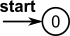
\includegraphics[width=4em]{transition_diagram_start}} &  The transition diagram always begins in the \emph{start state} before any input symbols have been read. \\
		\hline
		\raisebox{-.8\height}{
\includegraphics[width=5em]{transition_diagram_other}} &  The transition labelled with \textbf{other} is traversable when no other transition is traversable. \\
		\hline
		\raisebox{-.7\height}{
\includegraphics[width=1.7em]{transition_diagram_accept_state}} & The \emph{accepting state} (or final) indicates that a lexeme has been found (between pointers \code{lexemeBegin} and \code{forward}).
 \\
		\hline
		\raisebox{-\height}{
\includegraphics[width=2em]{transition_diagram_retract_state}} & If the lexeme does not include the symbol that got us to the accepting state, it is necessary to \emph{retract} the \code{forward} pointer by one position. \\
		\hline
	\end{tabularx}
	\end{small}
\end{frame}

\begin{frame}{Problem with Identifiers and Keywords}
	\begin{itemize}
	\item The transition diagram that recognizes the identifiers is:
	\vfill
		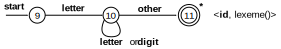
\includegraphics[width=\linewidth]{transition_diagram_identifier}
	\vfill
	\item \code{lexeme()} replies the current lexeme (between \code{lexemeBegin} and \code{forward} pointers).
	\end{itemize}
	\vfill
	\alertbox{Recognizing keywords and identifiers presents a specific problem:
keywords are not identifiers even though they look like identifiers.}
\end{frame}

%allowframebreaks
\begin{frame}{Solving the Problem with Identifiers and Keywords}
	There are two ways that we can handle reserved words that look like identifiers:
	\begin{enumerate}
	\item Install the keywords in the symbol table initially. A field of the symbol-table entry indicates that these strings are never ordinary identifiers.
		\begin{itemize}
		\item \code{installID()} places the identifier in the symbol table if it is not already there and returns a pointer to the symbol-table entry.
		\item \code{getToken()} replies the token that is corresponding to the lexeme, or \tok{id} otherwise.
		\end{itemize}
		\vfill
		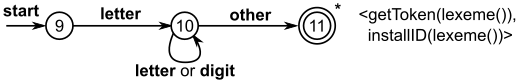
\includegraphics[width=\linewidth]{transition_diagram_identifier_keyword}
	\item Create a separate transition diagram for each keyword.
		\begin{itemize}
		\item If we adopt this approach, then we must prioritize the tokens so that the reserved-word tokens are recognized in preference to id, when the lexeme matches both patterns.
		\item This approach is less used than the previous approach when the lexical analyzer is written by hand.
		\end{itemize}
	\end{enumerate}
\end{frame}

\subsubsection{Implementation of a Lexical Analyzer based on Transition Diagrams}

\tableofcontentslide[sections={2-5},sectionstyle={show/shaded},subsectionstyle={show/shaded/hide},subsubsectionstyle={show/shaded/hide/hide}]

\begin{frame}{Implementation of a Lexical Analyzer}
	\begin{itemize}
	\item There are several ways that a collection of transition diagrams can be used to build a lexical analyzer.
	\vfill
	\item We may assume a variable state holding the number of the current state for a transition diagram.
	\vfill
	\item Each transition diagram is simulated by a piece of code inside a function.
	\vfill
	\item The code of a state is itself a switch statement or a multiway branch that determines the next state by reading and examining the next input character.
	\end{itemize}
\end{frame}

\begin{frame}[fragile]{Example of Code for the Token \tok{relop}}
	\begin{lstlisting}[language=Java]
	Token getRelop() { /* return null on failure */
	  char c;
	  Token token = new Token(Tag.RELOP);
	  while (true) { /* repeat until a return or failure */
	    switch(state) {
	    case 0: 
	      c = nextChar();
	      if (c=='<') state = 1;
	      else if (c=='=') state = 5;
	      else if (c=='>') state = 6;
	      else return null; /* lexeme is not a relop */
	      break;
	    case 1: ...
	    case 8:
	      retract();
	      token.attribute = "GT";
	      return token;
	    default: return null;
	    }
	  }
	}
	\end{lstlisting}
\end{frame}

%allowframebreaks
\begin{frame}{Combine Transition Diagrams}
	To build the entire lexical analyzer, the codes for simulating the transition diagrams may be arranged in different ways.
	\begin{enumerate}
	\item We could arrange for the transition diagrams for each token to be tried sequentially.
		\begin{itemize}
		\item Then when the function is replying null (failure), the pointer forward is reset and the next transition diagram is started.
		\item This approach allows us to use the transition diagrams for the individual keywords.
		\item We have only to use these before we use the diagram for id, in order the keywords to be reserved words.
		\end{itemize}
	\item We could run the various transition diagrams ``in parallel''.
		\begin{itemize}
		\item If we use this strategy, we must be careful to resolve the case where one diagram finds a lexeme that matches its pattern, while one or more other diagrams are still able to process input.
		\item The normal strategy is to take the longest prefix of the input that matches any pattern.
		\end{itemize}
	\item The preferred approach is to combine all the transition diagrams into one.
		\begin{itemize}
		\item We allow the transition diagram to read input until there is no possible next state, and then take the longest lexeme that matched any pattern.
		\item The problem of combining transition diagrams for several tokens is complex. The easiest way to solve this problem is to study how lexical-analyzer generators, such as Lex or Flex, are working.	
		\end{itemize}
	\end{enumerate}
\end{frame}

\section[Generators of lexical analyser]{Writing a lexical analyzer with Lex, Flex, JFlex, JavaCC}

\tableofcontentslide[sections={1-5},sectionstyle={show/shaded},subsectionstyle={show/show/hide},subsubsectionstyle={hide/hide/hide/hide}]

\subsection{Generators of Lexical Analyser}

\sidecite{Lesk.1975}
\begin{frame}{Generators of Lexical Analyser}
	\begin{itemize}
	\item Several tools allow to generate a lexical analyzer by specifying regular expressions to describe the patterns for the tokens.
	\item This section introduces the tool Lex, and its more recent implementation Flex (dedicated to compilers written in C or C++).
	\item The input notation is the Lex language.
	\end{itemize}
	\vfill
	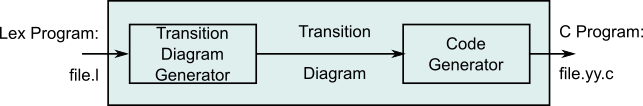
\includegraphics[width=\linewidth]{lex_tool}
\end{frame}

\subsection{Use of Lex}

\tableofcontentslide[sections={1-5},sectionstyle={show/shaded},subsectionstyle={show/shaded/hide},subsubsectionstyle={hide/hide/hide/hide}]

\figureslide{Process of Lex}{lex_process}

\begin{frame}{Key points to Implement main.c}
	\begin{itemize}
	\item The normal use of the program generated by the Lex compiler is as a \emph{subroutine} of the parser.
	\vfill
	\item \emph{The lexical analyzer is a C function} that returns an integer, which is a code for one of the possible token names.
	\vfill
	\item The attribute value, whether it another numeric code, a pointer to the symbol table, or nothing, is placed in a global variable \code{yylval} (shared between the lexical analyzer and the parser).
	\end{itemize}
\end{frame}

\subsection{Lex program}

\tableofcontentslide[sections={1-5},sectionstyle={show/shaded},subsectionstyle={show/shaded/hide},subsubsectionstyle={hide/hide/hide/hide}]

\begin{frame}[t,fragile]{Structure of a Lex program}
	\begin{itemize}
	\item A Lex program has the following form:
		\begin{lstlisting}[language=C]
		Declarations
		%%
		Translation rules
		%%
		Auxiliary functions
		\end{lstlisting}
	\end{itemize}
	\only<1>{\begin{block}{Declarations}
		\begin{itemize}
		\item declarations of variables,
		\item manifest constants: identifiers declared to stand for a constant, eg. the name of a token,
		\item regular definitions.
		\end{itemize}
	\end{block}}
	\only<2>{\begin{block}{Translation rules}
		\begin{itemize}
		\item have the form:
			\begin{center}
				\code{Pattern \{ Action \}}
			\end{center}
		\item Each pattern is a regular expression, which may use the regular definitions of the declaration section.
		\item The actions are fragments of code, usually in C.
		\item The first rule, which is matching, is used.
		\end{itemize}
	\end{block}}
	\only<3>{\begin{block}{Auxiliary functions}
		\begin{itemize}
		\item holds whatever additional functions are used in the actions.
		\end{itemize}
	\end{block}}
\end{frame}

\begin{frame}[fragile]{Example of a Lex Program: declarations}
	\begin{lstlisting}[language=C]
	%{
	  /* definitions of manifest constants, if not already
	     declared in the parser files (yacc) */
	  enum { LT, LE, EQ, NE, GT, GE	} RelopId;
	  enum { IF, THEN, ELSE, ID, NUMBER, RELOP } TokenName;
	%}
	/* regular expressions */
	delim   [ \t\n]
	ws      {delim}+
	letter  [A-Za-z]
	digit   [0-9]
	id      {letter}({letter}|{digit})*
	number  {digit}+(\.{digit}+)?([Ee][+-]?{digit}+)?
	%%
	\end{lstlisting}
\end{frame}

\begin{frame}[fragile]{Example of a Lex Program: translation rules}
	\begin{lstlisting}[language=C]
	{ws}      { /* no action and no return */ }
	if        { return IF; }
	then      { return THEN; }
	else      { return ELSE; }
	{id}      { yylval = (int)installID(); return ID; }
	{number}  { yylval = (int)installNumber(); return NUMBER; }
	"<"       { yylval = LT; return RELOP; }
	"<="      { yylval = LE; return RELOP; }
	"="       { yylval = EQ; return RELOP; }
	"<>"      { yylval = NE; return RELOP; }
	">"       { yylval = GT; return RELOP; }
	">="      { yylval = GE; return RELOP; }
	%%
	\end{lstlisting}
\end{frame}

\begin{frame}[fragile]{Example of a Lex Program: auxiliary functions}
	\begin{lstlisting}[language=C]
	int installID() {
	  /* function to install the lexeme, whose first
	     character is pointed to by yytext, and whose
	     length is yyleng, into the symbol table and
	     return a pointer thereto */
	}
	int installNumber() {
	  /* similar to installID, but puts numerical.
	     Constants into a separate table */
	}
	\end{lstlisting}
\end{frame}

\begin{frame}{Conflict Resolution with Lex}
	Two rules are used by Lex to decide on the proper lexeme to select, when several prefixes of the input match one or more patterns:
	\vfill
	\begin{enumerate}
	\item Always prefer a longer prefix to a shorter prefix.
	\vfill
	\item If the longest possible prefix matches two or more patterns, prefer the pattern listed first in the Lex program.
	\end{enumerate}
\end{frame}

\begin{frame}{Lookahead Operator}
	\begin{description}
	\item Lex automatically reads one character ahead of the last character that forms the selected lexeme, and then retracts the input so only the lexeme itself is consumed from the input.
	\vfill
	\item[Problem] Sometimes, we want a certain pattern to be matched to the input only when it is followed by a certain other characters.
	\vfill
	\item[Solution] use the character "\code{/}" in the pattern to indicate the end of the part of the pattern that matches the lexeme.
		\begin{itemize}
		\item \code{a / b} means ``a followed by b'' (a and b are regular expressions) 
		\item The additional pattern (b) is not consumed from the input in the lexical analyzer point-of-view.
		\end{itemize}
	\end{description}
\end{frame}

\subsection{Java generators}

\tableofcontentslide[sections={1-5},sectionstyle={show/shaded},subsectionstyle={show/shaded/hide},subsubsectionstyle={hide/hide/hide/hide}]

\begin{frame}[fragile]{JLex}
	\begin{itemize}
	\item Several implementations of lexical-analyzer generators provides Java source code.
	\vfill
	\item JLex is a lexical analyzer generator, written for Java, in Java.
	\item JLex is based upon the Lex lexical analyzer generator model $\Rightarrow$ \alert{the input file is the similar as the one for Lex, but not the same}.
		\begin{lstlisting}[language=C]
		User code
		%%
		JLex directives
		%%
		Translation rules
		\end{lstlisting}
	\end{itemize}
	\vfill
	\begin{center}
	\url{http://www.cs.princeton.edu/~appel/modern/java/JLex/}
	\end{center}
\end{frame}

\begin{frame}[fragile]{JLex Program}
	\begin{description}
	\item[User code] copied verbatim into the lexical analyzer source file. 
	\item[JLex directives] explained in the online documentation.
	\item[Translation rules] series of rules for breaking the input stream into tokens. \\
		Each rule has three distinct parts: the optional state list, the regular expression, and the associated action:
		\begin{center}
			\code{[{\textless}states{\textgreater}] {\textless}expression{\textgreater} \{ {\textless}action{\textgreater} \}}
		\end{center}
	\end{description}
	\vfill
	\begin{lstlisting}[language=C]
	User code
	%%
	JLex directives
	%%
	Translation rules
	\end{lstlisting}
\end{frame}

\begin{frame}{JFLex}
	\begin{itemize}
	\item JFLex  is a lexical analyzer generator, written for Java, in Java.
	\vfill
	\item It is a rewrite of JLex with extended features (as for Flex/Lex implementations).
	\end{itemize}
	\vfill
	\begin{center}
	\url{http://www.jflex.de}
	\end{center}
\end{frame}

\begin{frame}{JavaCC}
	\begin{itemize}
	\item Java Compiler Compiler (JavaCC) is the most popular parser generator for use with Java applications.
	\vfill
	\item Even if JavaCC is a parser, it includes a lexical analyzer in a transparent way.
	\vfill
	\item The lexical specifications such as regular expressions, strings, etc. and the grammar specifications (the BNF) are both written together in the same file.
	\vfill
	\item \emph{JavaCC is detailed in Chapter~\ref{chap:syntax_analysis}.}
	\end{itemize}
	\vfill
	\begin{center}
	\url{http://javacc.java.net}
	\end{center}
\end{frame}

\section[Lexical analyzer by hand]{Writing a lexical analyzer by hand}

\tableofcontentslide[sectionstyle={show/shaded},subsectionstyle={show/show/hide},subsubsectionstyle={hide/hide/hide/hide}]

\sidecite{Aho.1990, Hopcroft.2006}
\begin{frame}{Lexical Analyzer by Hand}
	To go deeper in how a program like Lex turns its input program into a lexical analyzer, the formalism called ``\Emph{finite automata}'' is at the heart of this transition.
\end{frame}

\subsection{Finite automata}

\sidecite{McCullough.1943}
\begin{frame}{Finite Automata}
	\begin{itemize}
	\item Finite automata are recognizers: they say ``yes'' or ``no'' about each possible input string.
	\vfill
	\item Finite automata come in two flavors:
		\begin{description}
		\item[Nondeterministic finite automata] NFA have no restrictions on the labels of their edges.
		\item[Deterministic finite automata] DFA have, for each state, and for each symbol of its input alphabet exactly one edge with that symbol leaving that state.
		\end{description}
	\vfill
	\item NFA and DFA are represented by \emph{transition graphes}.
	\item \emph{Similar to transition diagram}, except the same label can label edges from one state, and an edge may be labeled by $\epsilon$.
	\end{itemize}
\end{frame}

\subsubsection{Nondeterministic finite automata}

\tableofcontentslide[sections={1-5},sectionstyle={show/shaded},subsectionstyle={show/shaded/hide},subsubsectionstyle={show/show/hide/hide}]

\begin{frame}{Nondeterministic Finite Automata}
	A nondeterministic finite automata (NFA) consists of:
	\begin{enumerate}
	\item A finite set of states $S$.
	\vfill
	\item A set of input symbols $\Sigma$, the input alphabet. \\
		We assumed that $\epsilon$ is never a member of $\Sigma$.
	\vfill
	\item A transition function that gives, for each state, and for each symbol in $\Sigma\cup\{\epsilon\}$ a set of next states.
	\vfill
	\item A state $s_0$ from $S$ that is the start state or initial state.
	\vfill
	\item A set of states $F \subseteq S$, that are the accepting states or final states.
	\end{enumerate}
\end{frame}

\pgfdeclareimage[width=.7\paperwidth]{nfa_example}{./chapters/chapter2/imgs/auto/nfa_example}

\begin{frame}{Example of a NFA}
	\begin{itemize}
	\item The regular expression ``$(a|b)*abb$'' is described by the following NFA:
	\end{itemize}
	\vfill
	\begin{center}
	\pgfuseimage{nfa_example}
	\end{center}
\end{frame}

\begin{frame}{Running NFA on a String}
	\begin{itemize}
	\item An NFA accepts input strings \code{x} iff there is some path, such that the symbols along the path spell out \code{x}.
	\vfill
	\item Note that $\epsilon$ labels are ignored in the path.
	\vfill
	\item The language accepted by an NFA is the set of strings that have a path in the NFA.
	\end{itemize}
\end{frame}

\sidecite{Huffman.1954, Moore.1956, Thompson.1968}
\begin{frame}[fragile]{Algorithm for Simulating a NFA}
	\begin{myalgorithm}\smaller
	\SetKwFunction{epsilonclosure}{\ensuremath{\epsilon}-closure}
	\SetKwFunction{nextchar}{nextChar}
	\SetKwFunction{move}{move}
	\Input{An input string \code{x} terminated by \kw{eof} character. A NFA $N$ with start state $s_0$, accepting states $F$, and transition function move.}
	\Output{Answer ``yes'' if $N$ accepts \code{x}; ``no'' otherwise.}
	\Method{The algorithm keeps a set of current states $S$, those that are reached from $s_0$ following a path labeled by the inputs read so far. If $c$ is the next input character, read by the function nextChar, then we first compute \move($S$,$c$) and then close that set using \epsilonclosure.}
	\BlankLine
	\Begin{
		$S$ \affect \epsilonclosure($s_0$)\;
		$c$ \affect \nextchar\;
		\While{$c\neq\kw{eof}$}{
			$S$ \affect \epsilonclosure(\move($S$,$c$))\;
			$c$ \affect \nextchar\;
		}
		\Return $S \cap F \neq \emptyset$\;
	}
	\end{myalgorithm}
\end{frame}

\begin{frame}{Functions in the Algorithm}
	\begin{tabularx}{\linewidth}{|l|X|}
	\hline
	\tabularheading\chead{Operation}&\chead{Description}\\
	\hline
	$\epsilon$-closure($s$) & Set of NFA states reachable from NFA state $s$ on $\epsilon$-transitions alone. \\
	$\epsilon$-closure($T$) & Set of NFA states reachable form some NFA state $s$ in set $T$ on $\epsilon$-transitions alone. \\
	move($T$,$a$) & Set of NFA states to which there is a transition on input symbol a from some state $s$ in $T$. \\ 
	\hline
	\end{tabularx}
\end{frame}

\begin{frame}[t,fragile]{Example of NFA Simulation}
	\only<1>{\putat(-30,-132){\pgfuseimage{rightarrow}}}
	\only<2>{\putat(-30,-143){\pgfuseimage{rightarrow}}}
	\only<3,5,7,9,11,13,15>{\putat(-30,-164){\pgfuseimage{rightarrow}}}
	\only<4,6,8,10,12,14,16>{\putat(-30,-175){\pgfuseimage{rightarrow}}}
	\only<17>{\putat(-30,-196){\pgfuseimage{rightarrow}}}
	Let the input: "abababb"
	\begin{center}
	\pgfuseimage{nfa_example}
	\end{center}
	\begin{columns}
		\begin{column}[t]{.5\linewidth}
			\raisebox{-\height}{\begin{myalgorithm}\footnotesize
			\SetKwFunction{epsilonclosure}{\ensuremath{\epsilon}-closure}
			\SetKwFunction{nextchar}{nextChar}
			\SetKwFunction{move}{move}
			\Begin{
				$S$ \affect \epsilonclosure($s_0$)\;
				$c$ \affect \nextchar\;
				\While{$c\neq\kw{eof}$}{
					$S$ \affect \epsilonclosure(\move($S$,$c$))\;
					$c$ \affect \nextchar\;
				}
				\Return $S \cap F \neq \emptyset$\;
			}
			\end{myalgorithm}}
		\end{column}
		\begin{column}[t]{.5\linewidth}
			\begin{example}\smaller
			\only<1>{	$S = \{ 0 \}$\\
					foward: \texttt{abababb}}
			\only<2>{	$S = \{ 0 \}$\\
					$c = \texttt{a}$\\
					foward: \texttt{bababb}}
			\only<3>{	$S = \{ 0 \}$\\
					$c = \texttt{a}$\\
					move$(\{0\},\texttt{a})=\{0,1\}$\\
					$\epsilon$-closure$(\{0,1\}) = \{0,1\}$\\
					$S' = \{0,1\}$}
			\only<4>{	$S = \{0,1\}$\\
					$c = \texttt{b}$\\
					foward: \texttt{ababb}}
			\only<5>{	$S = \{0,1\}$\\
					$c = \texttt{b}$\\
					move$(\{0,1\},\texttt{b})=\{0,2\}$\\
					$\epsilon$-closure$(\{0,2\}) = \{0,2\}$\\
					$S' = \{0,2\}$}
			\only<6>{	$S = \{0,2\}$\\
					$c = \texttt{a}$\\
					foward: \texttt{babb}}
			\only<7>{	$S = \{0,2\}$\\
					$c = \texttt{a}$\\
					move$(\{0,2\},\texttt{a})=\{0\}$\\
					$\epsilon$-closure$(\{0\}) = \{0\}$\\
					$S' = \{0\}$}
			\only<8>{	$S = \{0\}$\\
					$c = \texttt{b}$\\
					foward: \texttt{abb}}
			\only<9>{	$S = \{0\}$\\
					$c = \texttt{b}$\\
					move$(\{0\},\texttt{b})=\{0\}$\\
					$\epsilon$-closure$(\{0\}) = \{0\}$\\
					$S' = \{0\}$}
			\only<10>{	$S = \{0\}$\\
					$c = \texttt{a}$\\
					foward: \texttt{bb}}
			\only<11>{	$S = \{0\}$\\
					$c = \texttt{a}$\\
					move$(\{0\},\texttt{a})=\{0,1\}$\\
					$\epsilon$-closure$(\{0,1\}) = \{0,1\}$\\
					$S' = \{0,1\}$}
			\only<12>{	$S = \{0,1\}$\\
					$c = \texttt{b}$\\
					foward: \texttt{b}}
			\only<13>{	$S = \{0,1\}$\\
					$c = \texttt{b}$\\
					move$(\{0,1\},\texttt{b})=\{0,2\}$\\
					$\epsilon$-closure$(\{0,2\}) = \{0,2\}$\\
					$S' = \{0,2\}$}
			\only<14>{	$S = \{0,2\}$\\
					$c = \texttt{b}$\\
					foward: \kw{eof}}
			\only<15>{	$S = \{0,2\}$\\
					$c = \texttt{b}$\\
					move$(\{0,2\},\texttt{b})=\{0,3\}$\\
					$\epsilon$-closure$(\{0,3\}) = \{0,3\}$\\
					$S' = \{0,3\}$}
			\only<16>{	$S = \{0,3\}$\\
					$c = \kw{eof}$}
			\only<17>{	$S = \{0,2\}$\\
					$F = \{3\}$\\
					$S \cap F = \{0,3\}\cap\{3\} = \{3\}$\\
					Return ``true''}
			\end{example}
		\end{column}
	\end{columns}
\end{frame}

\subsubsection{Deterministic finite automata}

\tableofcontentslide[sections={1-5},sectionstyle={show/shaded},subsectionstyle={show/shaded/hide},subsubsectionstyle={show/shaded/hide/hide}]

\begin{frame}{Deterministic Finite Automata}
	\begin{itemize}
	\item A deterministic finite automata (DFA) is a special case of an NFA where:
		\begin{enumerate}
		\item There are no moves on input $\epsilon$, and
		\item For each state $s$ and input symbol \texttt{a}, there is exactly one edge out of $s$ labeled \texttt{a}.
		\end{enumerate}
	\vfill
	\item While the NFA is used to recognize the strings of a language, the DFA is a simple and concrete algorithm for recognizing strings.
	\vfill
	\item Every regular expression and every NFA can be converted to a DFA accepting the same language.
	\vfill
	\item \emph{The lexical analyzers are built upon DFA.}
	\end{itemize}
\end{frame}

\pgfdeclareimage[width=.7\paperwidth]{dfa_example}{./chapters/chapter2/imgs/auto/dfa_example}

\begin{frame}{Example of a DFA}
	\begin{itemize}
	\item The regular expression ``$(a|b)*abb$'' is described by the following DFA:
	\end{itemize}
	\vfill
	\begin{center}
	\pgfuseimage{dfa_example}
	\end{center}
\end{frame}

\begin{frame}[fragile]{Algorithm for Simulating a DFA}
	\begin{myalgorithm}\smaller
	\SetKwFunction{nextchar}{nextChar}
	\SetKwFunction{move}{move}
	\Input{An input string \code{x} terminated by \kw{eof} character. A DFA $D$ with start state $s_0$, accepting states $F$, and transition function move.}
	\Output{Answer ``yes'' if $D$ accepts \code{x}; ``no'' otherwise.}
	\Method{Apply algorithm on \code{x}. The function \move($s$,$c$) gives the state to which there is an edge from state $s$ on input $c$. The function \nextchar returns the next character of the input string \code{x}.}
	\BlankLine
	\Begin{
		$s$ \affect $s_0$\;
		$c$ \affect \nextchar\;
		\While{$c\neq\kw{eof}$}{
			$s$ \affect \move($s$,$c$)\;
			$c$ \affect \nextchar\;
		}
		\Return $s \in F$\;
	}
	\end{myalgorithm}
\end{frame}

\begin{frame}[t,fragile]{Example of DFA Simulation}
	\only<1>{\putat(-30,-132){\pgfuseimage{rightarrow}}}
	\only<2>{\putat(-30,-143){\pgfuseimage{rightarrow}}}
	\only<3,5,7,9,11,13,15>{\putat(-30,-164){\pgfuseimage{rightarrow}}}
	\only<4,6,8,10,12,14,16>{\putat(-30,-175){\pgfuseimage{rightarrow}}}
	\only<17>{\putat(-30,-196){\pgfuseimage{rightarrow}}}
	Let the input: "abababb"
	\begin{center}
	\pgfuseimage{dfa_example}
	\end{center}
	\begin{columns}
		\begin{column}[t]{.5\linewidth}
			\raisebox{-\height}{\begin{myalgorithm}\footnotesize
			\SetKwFunction{nextchar}{nextChar}
			\SetKwFunction{move}{move}
			\Begin{
				$s$ \affect $s_0$\;
				$c$ \affect \nextchar\;
				\While{$c\neq\kw{eof}$}{
					$s$ \affect \move($s$,$c$)\;
					$c$ \affect \nextchar\;
				}
				\Return $s \in F$\;
			}
			\end{myalgorithm}}
		\end{column}
		\begin{column}[t]{.5\linewidth}
			\begin{example}\smaller
			\only<1>{	$s = 0$\\
					foward: \texttt{abababb}}
			\only<2>{	$s = 0$\\
					$c = \texttt{a}$\\
					foward: \texttt{bababb}}
			\only<3>{	$s = 0$\\
					$c = \texttt{a}$\\
					move$(0,\texttt{a}) = 1$\\
					$s' = 1$}
			\only<4>{	$s = 1$\\
					$c = \texttt{b}$\\
					foward: \texttt{ababb}}
			\only<5>{	$s = 1$\\
					$c = \texttt{b}$\\
					move$(1,\texttt{b}) = 2$\\
					$s' = 2$}
			\only<6>{	$s = 2$\\
					$c = \texttt{a}$\\
					foward: \texttt{babb}}
			\only<7>{	$s = 2$\\
					$c = \texttt{a}$\\
					move$(2,\texttt{a}) = 1$\\
					$s' = 1$}
			\only<8>{	$s = 1$\\
					$c = \texttt{b}$\\
					foward: \texttt{abb}}
			\only<9>{	$s = 1$\\
					$c = \texttt{b}$\\
					move$(1,\texttt{b}) = 2$\\
					$s' = 2$}
			\only<10>{	$s = 2$\\
					$c = \texttt{a}$\\
					foward: \texttt{bb}}
			\only<11>{	$s = 2$\\
					$c = \texttt{a}$\\
					move$(2,\texttt{a}) = 1$\\
					$s' = 1$}
			\only<12>{	$s = 1$\\
					$c = \texttt{b}$\\
					foward: \texttt{b}}
			\only<13>{	$s = 1$\\
					$c = \texttt{b}$\\
					move$(1,\texttt{b}) = 2$\\
					$s' = 2$}
			\only<14>{	$s = 2$\\
					$c = \texttt{b}$\\
					foward: \kw{eof}}
			\only<15>{	$s = 2$\\
					$c = \texttt{b}$\\
					move$(2,\texttt{b}) = 3$\\
					$s' = 3$}
			\only<16>{	$s = 3$\\
					$c = \kw{eof}$}
			\only<17>{	$s = 3$\\
					$F = \{3\}$\\
					Return ``true''}
			\end{example}
		\end{column}
	\end{columns}
\end{frame}

\subsubsection{From regular expression to NFA}

\tableofcontentslide[sections={1-5},sectionstyle={show/shaded},subsectionstyle={show/shaded/hide},subsubsectionstyle={show/shaded/hide/hide}]

%allowframebreaks
\sidecite{McNaughton.1960, Aho.1988, Thompson.1968}
\begin{frame}{Algorithm of McNaughton-Yamada-Thompson}
	\begin{description}
	\item[INPUT] A regular expression $r$ over alphabet $S$.
	\item[OUTPUT] An NFA $N$ accepting $L(r)$.
	\item[METHOD] Begin by parsing $r$ into its constituent subexpressions. The rules for constructing an NFA consist of basis rules for handling subexpressions with no operators, and inductive rules for a constructing larger NFA from the NFAs for the immediate subexpressions of a given expression.
	\vspace{1em}
	\item[BASIS 1] For each $\epsilon$ in $r$, construct the following NFA:
				\begin{center}
				
\includegraphics[width=.5\linewidth]{re_nfa_epsilon}
				\end{center}
	\item[BASIS 2] For any subexpression $a$ in $\Sigma$, construct the following NFA:
				\begin{center}
				
\includegraphics[width=.5\linewidth]{re_nfa_expr}
				\end{center}
			\alertbox*{Note that in both of the basis constructions, we construct a distinct NFA, with new states, for every occurrence of $\epsilon$ or some $a$ as a subexpression of $r$.}
	\item[INDUCTION 1] Suppose $r = s|t$. Then $N(r)$ is:
			\begin{center}
				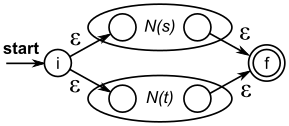
\includegraphics[width=.7\linewidth]{re_nfa_or}
			\end{center}
	\vspace{1em}
	\item[INDUCTION 2] Suppose $r = st$. Then $N(r)$ is:
		\begin{center}
			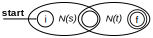
\includegraphics[width=.6\linewidth]{re_nfa_seq}
		\end{center}
	\item[INDUCTION 3] Suppose $r = s*$. Then $N(r)$ is:
		\begin{center}
			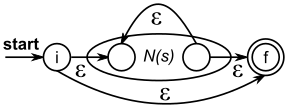
\includegraphics[width=.7\linewidth]{re_nfa_loop}
		\end{center}
	\vspace{1em}
	\item[INDUCTION 4] Suppose $r = (s)$. Then $N(r)=N(s)$.
	\end{description}
\end{frame}

\animatedslide{Example of Conversion of $(a|b)*abb$}{re_nfa_example}{width=\linewidth}

\subsubsection{From NFA to DFA}

\tableofcontentslide[sections={1-5},sectionstyle={show/shaded},subsectionstyle={show/shaded/hide},subsubsectionstyle={show/shaded/hide/hide}]

\begin{frame}{Converting NFA to DFA}
	\begin{itemize}
	\item The general idea behind the conversion is that each state of the constructed DFA corresponds to a set of NFA states.
	\vfill
	\item It is possible that the number of DFA states is exponential in the number of NFA states, which could lead to difficulties when we try to implement this DFA.
	\vfill
	\item The subset construction is an algorithm based on this idea. It is presented in the next slide.
	\end{itemize}
\end{frame}

\begin{frame}[fragile]{Algorithm for Converting NFA to DFA}
	\begin{myalgorithm}
	\Input{An NFA $N$.}
	\Output{A DFA $D$ accepting the same language $N$.}
	\Method{\begin{enumerate}
		\item The algorithm constructs a transition table $Dtran$ from $D$. Each state of $D$ is a set of NFA states, and we construct $Dtran$ so that $D$ will simulate ``in parallel'' all the possible moves $N$ can make on a given input string. \\
		\item The NDA may be built from the table $Dtran$.
		\end{enumerate}}
	\end{myalgorithm}
\end{frame}

\begin{frame}[fragile]{Building the Table $Dtran$}
	\begin{myalgorithm}\smaller
	\SetKwFunction{epsilonclosure}{\ensuremath{\epsilon}-closure}
	\SetKwFunction{move}{move}
	\Begin{
		$T$ \affect \epsilonclosure($s_0$)\;
		$Dstates$ \affect $\{ T \}$\;
		$Unmarked$ \affect $\{ T \}$\;
		\While{$\exists T \in Umarked$}{
			$Unmarked$ \affect $Unmarked \setminus \{T\}$\;
			\ForEach{input symbol $a$}{
				$U$ \affect \epsilonclosure(\move($T$,$a$))\;
				\If{$U \not\in DStates$}{
					$Dstates$ \affect $Dstates \cup \{U\}$\;
					$Unmarked$ \affect $Umarked \cup \{U\}$\;
				}
				$Dtran[T,a]$ \affect $U$\;
			}
		}
	}
	\end{myalgorithm}
\end{frame}

\pgfdeclareimage[width=.5\paperwidth]{nfa_full}{./chapters/chapter2/imgs/auto/nfa_full}
\pgfdeclareimage[width=.7\paperwidth]{dfa_full}{./chapters/chapter2/imgs/auto/dfa_full}

\begin{frame}[t]{Example of the Building of $Dtran$}\smaller
	Let consider the NFA for the regular expression $(a|b)*abb$.
	\begin{center}
		\pgfuseimage{nfa_full}
	\end{center}
	\begin{scriptsize}
	\begin{tabularx}{\linewidth}{|c|X|c|c|c|}
		\hline
		\tabularheading\chead{Label}&\chead{$Dstates$}&\chead{$\in Unmarked$}&\chead{\texttt{"a"}}&\chead{\texttt{"b"}}\\
		\hline
		\only<1->{A & $\{1,3,5,7,8\}$ & \only<1>{$\times$} & \only<2->{B} & \only<3->{C}\\\hline}
		\only<2->{B & $\{1,2,3,5,6,8,9\}$ & \only<2-3>{$\times$} & \only<4->{B} & \only<5->{D} \\\hline}
		\only<3->{C & $\{1,3,4,5,6,8\}$ & \only<3-5>{$\times$} & \only<6->{B} & \only<7->{C} \\\hline}
		\only<5->{D & $\{1,3,4,5,6,8,10\}$ & \only<4-8>{$\times$} & \only<8->{B} & \only<9->{E} \\\hline}
		\only<9->{E & $\{1,3,4,5,6,8,11\}$ & \only<9>{$\times$} & \only<10->{B} & \only<11>{C} \\\hline}
	\end{tabularx}
	\end{scriptsize}
	\vfill
	\begin{block}{\tiny Notes}\tiny
		\only<1>{	$T = \epsilon$-closure$(s_0) = \epsilon$-closure$(7) = \{1,3,5,7,8\}$}
		\only<2>{	$T = \{1,3,5,7,8\}$ and unmark $T$ \\
				$a = \texttt{"a"}$ \\
				$U = \epsilon$-closure$($move$(T,a)) = \epsilon$-closure$(\{2,9\}) = \{1,2,3,5,6,8,9\}$ \\
				$U$ is a new state (B), and $Dtran[T,a] = $B
		}
		\only<3>{	$T = \{1,3,5,7,8\}$ \\
				$a = \texttt{"b"}$ \\
				$U = \epsilon$-closure$($move$(T,a)) = \epsilon$-closure$(\{4\}) = \{1,3,4,5,6,8\}$ \\
				$U$ is a new state (C), and $Dtran[T,a] = $C
		}
		\only<4>{	$T = \{1,2,3,5,6,8,9\}$ and unmark $T$ \\
				$a = \texttt{"a"}$ \\
				$U = \epsilon$-closure$($move$(T,a)) = \epsilon$-closure$(\{2,9\}) = \{1,2,3,5,6,8,9\}$ \\
				$U$ is B, $Dtran[T,a] = $B
		}
		\only<5>{	$T = \{1,2,3,5,6,8,9\}$ \\
				$a = \texttt{"b"}$ \\
				$U = \epsilon$-closure$($move$(T,a)) = \epsilon$-closure$(\{4,10\}) = \{1,3,4,5,6,8,10\}$ \\
				$U$ is a new state (D), $Dtran[T,a] = $D
		}
		\only<6>{	$T = \{1,3,4,5,6,8\}$ and unmark $T$ \\
				$a = \texttt{"a"}$ \\
				$U = \epsilon$-closure$($move$(T,a)) = \epsilon$-closure$(\{2,9\}) = \{1,2,3,5,6,8,9\}$ \\
				$U$ is B, $Dtran[T,a] = $B
		}
		\only<7>{	$T = \{1,3,4,5,6,8\}$ \\
				$a = \texttt{"b"}$ \\
				$U = \epsilon$-closure$($move$(T,a)) = \epsilon$-closure$(\{4\}) = \{1,3,4,5,6,8\}$ \\
				$U$ is C, $Dtran[T,a] = $C
		}
		\only<8>{	$T = \{1,3,4,5,6,8,10\}$ and unmark $T$ \\
				$a = \texttt{"a"}$ \\
				$U = \epsilon$-closure$($move$(T,a)) = \epsilon$-closure$(\{2,9\}) = \{1,2,3,5,6,8,9\}$ \\
				$U$ is B, $Dtran[T,a] = $B
		}
		\only<9>{	$T = \{1,3,4,5,6,8,10\}$ \\
				$a = \texttt{"b"}$ \\
				$U = \epsilon$-closure$($move$(T,a)) = \epsilon$-closure$(\{4,11\}) = \{1,3,4,5,6,8,11\}$ \\
				$U$ is a new state (E), $Dtran[T,a] = $E
		}
		\only<10>{	$T = \{1,3,4,5,6,8,11\}$ and unmark $T$ \\
				$a = \texttt{"a"}$ \\
				$U = \epsilon$-closure$($move$(T,a)) = \epsilon$-closure$(\{2,9\}) = \{1,2,3,5,6,8,9\}$ \\
				$U$ is B, $Dtran[T,a] = $B
		}
		\only<11>{	$T = \{1,3,4,5,6,8,11\}$ \\
				$a = \texttt{"b"}$ \\
				$U = \epsilon$-closure$($move$(T,a)) = \epsilon$-closure$(\{4\}) = \{1,3,4,5,6,8\}$ \\
				$U$ is C, $Dtran[T,a] = $C
		}
	\end{block}
\end{frame}

\begin{frame}{Building the DFA from the Table $Dtran$}
	\vspace{1em}
	\begin{scriptsize}
	\begin{tabularx}{\linewidth}{|c|X|c|c|c|c|}
		\hline
		\tabularheading\chead{Label}&\chead{$Dstates$}&\chead{Init.}&\chead{Final}&\chead{\texttt{"a"}}&\chead{\texttt{"b"}}\\
		\hline
		A & $\{1,3,5,7,8\}$ & yes & $\emptyset$ & B & C \\\hline
		B & $\{1,2,3,5,6,8,9\}$ & no & $\emptyset$ & B & D \\\hline
		C & $\{1,3,4,5,6,8\}$ & no & $\emptyset$ & B & C \\\hline
		D & $\{1,3,4,5,6,8,10\}$ & no & $\emptyset$ & B & E \\\hline
		E & $\{1,3,4,5,6,8,11\}$ & no & $\{11\}$ & B & C \\\hline
	\end{tabularx}
	\end{scriptsize}
	\vfill
	\begin{center}
			\pgfuseimage{dfa_full}
	\end{center}
\end{frame}

\subsection{Building a Lexical Analyzer}

\tableofcontentslide[sections={1-5},sectionstyle={show/shaded},subsectionstyle={show/shaded/hide},subsubsectionstyle={show/show/hide/hide}]

\subsubsection{Pattern matching with NFA}

\begin{frame}[fragile]{Automaton based on NFA}
	\begin{itemize}
	\item To construct the automaton, we take each regular-expression pattern and converting it to an NFA.
	\vfill
	\item We need a single global automaton, so we combine all the NFA's into one by introducing a new start state.
	\vfill
	\item Let take the example:
		\begin{lstlisting}[language=C,basicstyle={\normalsize}]
		a        { do_Action1(); }
		abb      { do_Action2(); }
		a*b+     { do_Action3(); }
		\end{lstlisting}
	\end{itemize}
\end{frame}

\animatedslide[2-]{Example of the NFA Automaton}{complete_nfa_automaton}{width=\linewidth}

\begin{frame}{Running the NFA Automaton}
	\begin{itemize}
	\item The lexical analyzer reads the input from \code{lexemeBegin}.
	\item The NFA is evaluated according to the input pointed by the \code{forward} pointer.
	\vfill
	\item When the NFA simulation does not find any more state, we could find the longest validated lexeme: \begin{itemize}
		\item Look backwards in the sequence of sets of states, until accepting states were found.
		\item If found accepting states, replies the associated lexeme.
		\item Otherwise, there is a syntax error.
		\end{itemize}
	\end{itemize}
\end{frame}

\pgfdeclareimage[width=.7\paperwidth]{nfa_automaton_small}{./chapters/chapter2/imgs/auto/nfa_automaton_small}

\begin{frame}[t]{Example of Simulation of NFA}
	Let consider the input: \texttt{aaba}
	\begin{center}
		\pgfuseimage{nfa_automaton_small}\\
		\includeanimatedfigure[width=.8\linewidth]{nfa_automaton_exec}%
	\end{center}
	\putat(10,-180){\parbox[t]{.9\linewidth}{\normalsize\mdseries\normalcolor
		\begin{footnotesize}
		\only<1>{	Initially, the set of states contains the $\epsilon$-closure of the state $0$.}
		\only<2>{	Read \texttt{"a"} \\[-.5em]
				States: $\epsilon$-closure(move($\{0,1,3,7\}$, \texttt{"a"}))$ = \{ 2, 4, 7 \}$ \\[-.5em]
				State $2$ is a final state $\Rightarrow$ lexeme detected for pattern $a$
		}
		\only<3>{	Read \texttt{"a"} \\[-.5em]
				States: $\epsilon$-closure(move($\{2,4,7\}$, \texttt{"a"}))$ = \{ 7 \}$
		}
		\only<4>{	Read \texttt{"b"} \\[-.5em]
				States: $\epsilon$-closure(move($\{7\}$, \texttt{"b"}))$ = \{ 8 \}$ \\[-.5em]
				State $8$ is a final state $\Rightarrow$ lexeme detected for pattern $a*b+$
		}
		\only<5>{	Read \texttt{"a"} \\[-.5em]
				States: $\epsilon$-closure(move($\{8\}$, \texttt{"a"}))$ = \emptyset$ \\[-.5em]
				\emph{Simulation is done. Look backward.}
		}
		\end{footnotesize}
	}}
\end{frame}

\subsubsection{Pattern matching with DFA}

\tableofcontentslide[sections={1-5},sectionstyle={show/shaded},subsectionstyle={show/shaded/hide},subsubsectionstyle={show/shaded/hide/hide}]

\begin{frame}[fragile]{Automaton based on DFA}
	\begin{itemize}
	\item To construct the automaton, we take each regular-expression pattern and converting it to an DFA (directly or via a NFA).
	\vfill
	\item Within each DFA state, if there are one or more accepting NFA states, use the first pattern in the Lex program associated to these NFA states.
	\vfill
	\item Let take the example:
		\begin{lstlisting}[language=C,basicstyle={\normalsize}]
		a        { do_Action1(); }
		abb      { do_Action2(); }
		a*b+     { do_Action3(); }
		\end{lstlisting}
	\end{itemize}
\end{frame}

\pgfdeclareimage[width=.8\linewidth]{complete_dfa_automaton}{imgs/chapter2/complete_dfa_automaton}

\begin{frame}{Example of the DFA Automaton}
	\begin{center}
		\pgfuseimage{complete_dfa_automaton}
	\end{center}
	\vfill
	\begin{block}{\small Note}\small
	Both states $6$ and $8$ are final states for patterns ``$abb$'' and ``$a*b+$'', resp.
	Only the first in the Lex program is considered by the DNA.
	\end{block}
\end{frame}

\begin{frame}{Running the DFA Automaton}
	\begin{itemize}
	\item We use the DFA in a lexical analyzer much as we did with the NFA.
	\vfill
	\item We simulate the DFA until at some point there is no next state, or strictly speaking, the next state is $\emptyset$, the dead state corresponding to the empty set of NFA states.
	\vfill
	\item At that point, we go back through the sequence of states.
	\item As soon as an accepting DFA state is encountered, the associated action is performed.
	\end{itemize}
\end{frame}

\begin{frame}[t]{Example of Simulation of DFA}
	Let consider the input: \texttt{aaba}
	\begin{center}
		\resizebox{.4\linewidth}{!}{\pgfuseimage{complete_dfa_automaton}}
		\includeanimatedfigure[width=.8\linewidth]{dfa_automaton_exec}%
	\end{center}
	\putat(10,-160){\parbox[t]{.9\linewidth}{\normalsize\mdseries\normalcolor
		\only<1>{	
				\begin{footnotesize}
				Initially, the selected state is $(0137)$.
				\end{footnotesize}
		}
		\only<2>{	
				\begin{footnotesize}
				Read \texttt{"a"}. \\[-.5em]
				Pass the edge of the DFA, and update the current state. \\[-.5em]
				Because the state $2$ is a final state in the NFA, the state \\[-.5em]
				$(247)$ is marked.
				\end{footnotesize}
		}
		\only<3>{	
				\begin{footnotesize}
				Read \texttt{"a"}, and pass the edge.
				\end{footnotesize}
		}
		\only<4>{	
				\begin{footnotesize}
				Read \texttt{"b"}. \\[-.5em]
				Pass the edge of the DFA, and update the current state. \\[-.5em]
				Because the state $8$ is a final state in the NFA, the state $(8)$ is marked.
				\end{footnotesize}
		}
		\only<5>{	
				\begin{footnotesize}
				Read \texttt{"a"}. \\[-.5em]
				No state is accessible. \\[-.5em]
				\emph{Simulation is done. Look backward.}
				\end{footnotesize}
		}
	}}
\end{frame}

\section{Conclusion}

\tableofcontentslide[sectionstyle={show/shaded},subsectionstyle={hide/hide/hide},subsubsectionstyle={hide/hide/hide/hide}]

%allowframebreaks
\begin{frame}[t]{Key Concepts in the Chapter}
	\begin{description}\small
	\item[Tokens] The lexical analyzer scans the source program and produces as output a sequence of tokens, which are normally passed, one at a time to the parser.
	\item[Lexemes] Each time the lexical analyzer returns a token to the parser, is has an associated lexeme: the sequence of characters that the token represents.
	\item[Buffering] Because it is often necessary to scan ahead on the input in order to see where the next lexeme ends, it is necessary for the lexical analyzer to buffer the input.
	\item[Patterns] Each token has a pattern that describes which sequences of characters can form the lexemes corresponding to that token.
	\item[Regular Expressions] These expressions are commonly used to describe patterns. Regular expressions are built from single characters, using union, concatenation, and the Kleene closure.
	\item[Transition Diagram] The behavior of a lexical analyzer can be described with a transition diagram. The states of that diagram represent the history of the characters seen during the analysis. The edges between the states indicate the possible next characters.
	\item[Finite Automata] These are a formalization of transition diagrams. Accepting states indicates that a lexeme for a token has been found. Unlike transition diagrams, finite automata can make transitions on empty input as well as on input characters.
	\item[Deterministic Finite Automata] A DFA is a special kind of finite automata that has exactly one transition out from each state for each input symbol.
	\item[Nondeterministic Finite Automata] Automata that are not DFA are called nondeterministic.
	\item[Conversion Among Pattern Representations] It is possible to convert any regular expression to NFA, and to convert any NFA to DFA.
	\item[Lex] Family of software systems that are able to generate lexical analyzers from input specifications.
	\end{description}
\end{frame}

%allowframebreaks
\begin{frame}[t]{\bibname\ of the Chapter}%
	\tiny%
	\putbib[bibliographies/chapter2]%
\end{frame}%

\end{bibunit}
\end{graphicspathcontext}